%%%%%%%%%%%%%%%%%%%%%%% file template.tex %%%%%%%%%%%%%%%%%%%%%%%%%
%
% This is a template file for Web of Conferences Journal
%
% Copy it to a new file with a new name and use it as the basis
% for your article
%
%%%%%%%%%%%%%%%%%%%%%%%%%% EDP Science %%%%%%%%%%%%%%%%%%%%%%%%%%%%
%
%%%\documentclass[option]{webofc}
%%% "twocolumn" for typesetting an article in two columns format (default one column)
%
\documentclass{webofc}
\usepackage[varg]{txfonts}   % Web of Conferences font
%
% Put here some packages required or/and some personnal commands
%
%

\def\kbdstyle{\smaller\bfseries\ttfamily}
\newcommand{\kbd}[1]{{\kbdstyle #1}\xspace}
\newcommand{\code}[1]{\textcolor{blue!60!green}{\kbd{#1}}\xspace}
\newcommand{\pkg}[1]{\textcolor{purple!40!black!80!white}{\kbd{#1}}\xspace}
\newcommand{\cmd}[1]{\kbd{#1}\xspace}
\newcommand{\subst}[1]{\ensuremath{\langle\text{\textit{#1}}\rangle}}

\renewcommand{\bold}[1]{\textbf{#1}}
\newcommand{\italic}[1]{\textit{#1}}
\newcommand{\highlight}[1]{\red{#1}\xspace}
\newcommand{\subdued}[1]{\grey{#1}\xspace}
\newcommand{\minor}[1]{\grey{\smaller #1}}

\newcommand{\col}[1]{\column{#1\textwidth}}

%%%%%%%%%%%%%%%%%%

\newcommand{\secref}[1]{Sect.~\ref{#1}}
\newcommand{\tabref}[1]{Tab.~\ref{#1}}
\newcommand{\figref}[1]{Fig.~\ref{#1}}
\newcommand{\mini}{\mathop{\mbox{minimize}}}
\newcommand{\maxi}{\mathop{\mbox{maximize}}}
\newcommand{\amin}{\mathop{\mbox{argmin}}}
\newcommand{\amax}{\mathop{\mbox{argmax}}}
\newcommand{\st}{\mbox{subject to }}
\newcommand{\bmath}[1]{\mbox{\boldmath $ #1 $}}
\newcommand{\R}{\mathbb{R}}
\newcommand{\dps}{\displaystyle}
\newcommand{\p}{\bmath{p}}
%\newcommand{\p}{\ensuremath{\vec{p}\xspace}}
\newcommand{\phat}{\ensuremath{\hat{p}}\xspace}
\newcommand{\phisq}{\ensuremath{\phi^2}\xspace}
\newcommand{\phato}{\ensuremath{\hat{p}|\left\{w_\mathcal{O}\right\}\xspace}}
\newcommand{\pzero}{\ensuremath{\vec{p}_0}\xspace}
\newcommand{\pprime}{\ensuremath{\vec{p}'}\xspace}
\newcommand{\ptilde}{\ensuremath{\tilde{p}\xspace}}
\newcommand{\vptilde}{\ensuremath{\tilde{\vec{p}}}\xspace}
\renewcommand{\d}[1]{\ensuremath{\mathrm{d}#1}\xspace}
\newcommand{\nCr}[2]{\ensuremath{\parenths{\colvec{#1 \\ #2}}}\xspace}
\newcommand{\alphaS}{\ensuremath{\alpha_\text{s}}\xspace}
\newcommand{\alphaSMZ}{\ensuremath{\alpha_\text{s}(M_Z)}\xspace}
\newcommand{\pT}{\ensuremath{p_\mathrm{T}}\xspace}
\newcommand{\kT}{\ensuremath{k_\mathrm{T}}\xspace}

\newcommand{\qqbar}{\ensuremath{q\bar{q}}\xspace}
\newcommand{\QQbar}{\ensuremath{Q\bar{Q}}\xspace}
\newcommand{\ttbar}{\ensuremath{t\bar{t}}\xspace}
\newcommand{\bbbar}{\ensuremath{b\bar{b}}\xspace}
\newcommand{\ccbar}{\ensuremath{c\bar{c}}\xspace}
\newcommand{\ssbar}{\ensuremath{s\bar{s}}\xspace}

\newcommand{\tofrom}{\ensuremath{\leftrightarrow}}
\renewcommand{\to}{\ensuremath{\rightarrow}\xspace}
\newcommand{\To}{\ensuremath{\Rightarrow}\xspace}
\newcommand{\ToFrom}{\ensuremath{\Leftrightarrow}}
\newcommand{\tick}{\checkmark}

\newcommand{\Cxx}{C\!\,\raisebox{0.05\baselineskip}{++}\xspace}
\newcommand{\xx}{\!\,\raisebox{0.05\baselineskip}{++}\xspace}
\newcommand{\Fortran}{\textsc{Fortran}\xspace}

\newcommand{\eV}{\ensuremath{\text{e\kern-0.15ex{}V}}\xspace}
\newcommand{\MeV}{\ensuremath{\text{M\eV}}\xspace}
\newcommand{\GeV}{\ensuremath{\text{G\eV}}\xspace}
\newcommand{\TeV}{\ensuremath{\text{T\eV}}\xspace}

\begin{document}
%
\title{Teaching PROFESSOR new math}
%
% subtitle is optionnal
%
%%%\subtitle{Do you have a subtitle?\\ If so, write it here}

\author{
    \firstname{Anthony} \lastname{Austin}\inst{1}\fnsep\thanks{\email{apaustin@vt.edu}} \and
    \firstname{Sven} \lastname{Leyffer}\inst{2}\fnsep\thanks{\email{leyffer@mcs.anl.gov}} \and
    \firstname{Steven} \lastname{Mrenna}\inst{3}\fnsep\thanks{\email{mrenna@fnal.gov}} \and
    \firstname{Juliane} \lastname{M\"uller}\inst{4}\fnsep\thanks{\email{julianemueller@lbl.gov}} \and
    \firstname{Holger} \lastname{Schulz}\inst{3,5}\fnsep\thanks{\email{hschulz@fnal.gov}}
}

\institute{
           Virginia Tech \and
           Argonne National Laboratory \and
           Fermi National Accelerator Laboratory\and
           Lawrence Berkeley National Laboratory\and
            University of Cincinnati 
          }

\abstract{%
    The software package PROFESSOR~\cite{Buckley:2009bj} provides machinery to
    facilitate Monte-Carlo (MC) event-generator tuning.  The method is based on
    a numerical optimisation of a goodness-of-fit (GOF) measure defined between
    measured experimental data and MC predictions. As the latter are typically
    very expensive to evaluate, PROFESSOR replaces them with fast to evaluate
    surrogates. We present improvements to the method in the numerical
    optimisation as well as the surrogate construction. Firstly, we introduce
    an algorithm and implementation of a bi-level optimisation problem aimed at
    improving scenarios were the underlying physics model is unable to describe
    all data to the same accuracy. Secondly, we display our implementation of
    an algorithm for multivariate rational approximations which are superior to
    the previously used polynomial surrogates.
}
%
\maketitle

%
\section{Introduction}
\label{intro}
Monte-Carlo event generators are an essential tool for physics analyses. Their
predictions are used e.g. to estimate background contributions, to correct for
detector effects and ultimately test physics models against measured data. It
is therefore desirable to achieve particle simulations that are as precise as
possible. In the last decade tremendous success was achieved in the
perturbative regime of the underlying calculations. Realistic MC generators,
however, also contain physics in a regime where couplings are large and field
theory methods break down.  Programmes such as Pythia8~\cite{Sjostrand:2007gs}
implement non-perturbative aspects of the simulation by means of heuristic
models that introduce parameters that need to be adjusted to meaningful values
with the objective to reproduce nature with high fidelity.  This process, which
is commonly referred to as ``tuning'', is helped greatly by the existence of
tools like Rivet~\cite{Buckley:2010ar} which conveniently analyse the simulated
events to allow for immediate comparison with a trove of experimental data,
e.g.  in the form of a goodness-of-fit measure such as
\begin{equation}\label{eq:gof}
    \chi^2(p) = \sum\limits_b^{N_\text{bins}} \frac{\left[d_b - \text{MC}_b(p)\right]^2}{\sigma_b^2},
\end{equation}
where the sum runs over individual bins, $b$. The measured data is given by
$d_b$ and some uncertainty $\sigma_b$. The corresponding Monte-Carlo
prediction $\text{MC}_b(p)$ is dependent on model parameter points, $p$.  The
optimisation problem is defined such that we want to find the point $\hat{p}$
that minimises the expression in \eqref{eq:gof}. The computational cost
of running the MC generators for a given point $p$ range from minutes
to days, depending on the physics process. For most cases, this is too
expensive for numerical minimisations. PROFESSOR instead uses surrogates $f_b$
that are trained on a moderate number of $\text{MC}(p)$. The evaluation of
$f_b(p)$ is of the order of micro-seconds which is much more amenable for
numerical minimisation purposes.

In the best of all worlds, the models would be able to describe all measured
data with one set of parameter values. However, more often than not this is
not the case. Instead, specialised tunes are developed by biasing the
optimisation process to give more weight to certain datasets than others. This
process typically involves many iterations in a trial-and-error fashion. We
attempt to automate this procedure in \secref{sec-oopt} in a bi-level
formulation of the optimisation problem defined in \eqref{eq:gof}.

Although fairly robust and widely applicable, the multivariate polynomial approximations
used in PROFESSOR so far do have limitations if the true functional form of the
to be approximated data exhibits traits of rational functions. In \secref{sec-rapp}
we demonstrate our implementation of an algorithm for multivariate rational
approximations.


\subsection{Bi-level optimisation}
\label{sec-oopt}

The ``classical'' tuning problem can be
    \begin{itemize}
        \item Incompatible datasets and mismodelling in MC generator necessitate introduction of tuning weights $w_b$
        \item Adjusting the weights has so far been a manual procedure
        \item The user would iteratively run the ``inner optimisation`` and look at resulting plots
        \item We propose an automated procedure for this ''outer optimisation``:
            \begin{itemize}
                \item Write goodness-of-fit in terms of histograms/observables
                \item The parameter space is now the observable-weight space
                \item Inner optimisation yields best fit point, \phat, for given $$\left\{w_\mathcal{O}\right\}$$
                \item \phat is used to evaluate an objective function for the outer optimisation
            \end{itemize}
    \end{itemize}
$$
    \phisq(\p|\left\{w_\mathcal{O}\right\}) =
    \sum_{\mathcal{O}=1}^N w_\mathcal{O}^2 \cdot
    \sum_{b\in \mathcal{O}}
  \frac{ (f_b(\p) - \mathcal{R}_b)^2 }{   \Delta^2}
$$

    \begin{itemize}
        \item For given \phat, we can calculate the per-observable goodness-of fit
    \end{itemize}
$$
    \nu_\mathcal{O}(\phato) =
    \frac{1}{N_\text{bins}(\mathcal{O})}
    \sum_{b\in \mathcal{O}}
  \frac{ (f_b(\phato) - \mathcal{R}_b)^2 }{  \Delta^2}, \ {\cal O} =1,\ldots, N
$$
\begin{itemize}
    \item With $N$ such measures, we can calculate mean and standard deviation
\end{itemize}
$$%\begin{equation} 
 \mu(w_{\cal O}, \p^*) = \frac{1}{N}\sum_{{\cal O}=1}^N \nu_{\cal O}(w_{\cal O}, \p^*)
$$%\end{equation}	
$$% \begin{equation} 
 \sigma^2(w_{\cal O}, \p^*) = \frac{1}{N}\sum_{{\cal O}=1}^N \left[\nu_{\cal O}(w_{\cal O}, \p^*) -\mu(w_{\cal O}, \p^*)\right]^2
$$%\end{equation}	
    \begin{itemize}
            \item And construct an objective function to minimise
        \end{itemize}
$$% \begin{equation}
\min_{w_{\cal O}\in[0,1]} \lambda \mu(w_{\cal O}, \p^*) + \sigma^2(w_{\cal O}, \p^*),\quad \text{s.t. } \sum_{{\cal O}=1}^N w_{\cal O} =1.
$$%\end{equation}	


    \begin{itemize}
        \item Minimisation of portfolio objective is iterative
        \item We train a radial basis function and use it to walk through the weight space
        \item Convergence is fast but depends on initial guess $\to$ multi-start approach (that's ok since inner optimisation is really fast)
    \end{itemize}
    \begin{minipage}{.48\textwidth}%
        \begin{center}
            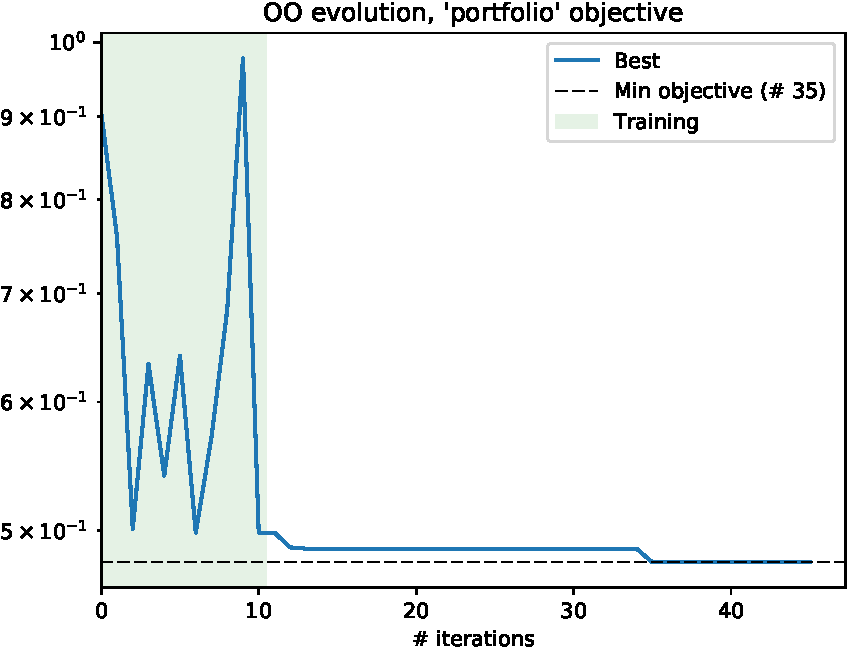
\includegraphics[width=.98\textwidth]{oo/chain-3-report.pdf}
        \end{center}
    \end{minipage}%
    \begin{minipage}{.04\textwidth}%
    \end{minipage}%
    \begin{minipage}{.48\textwidth}%
        \begin{center}
            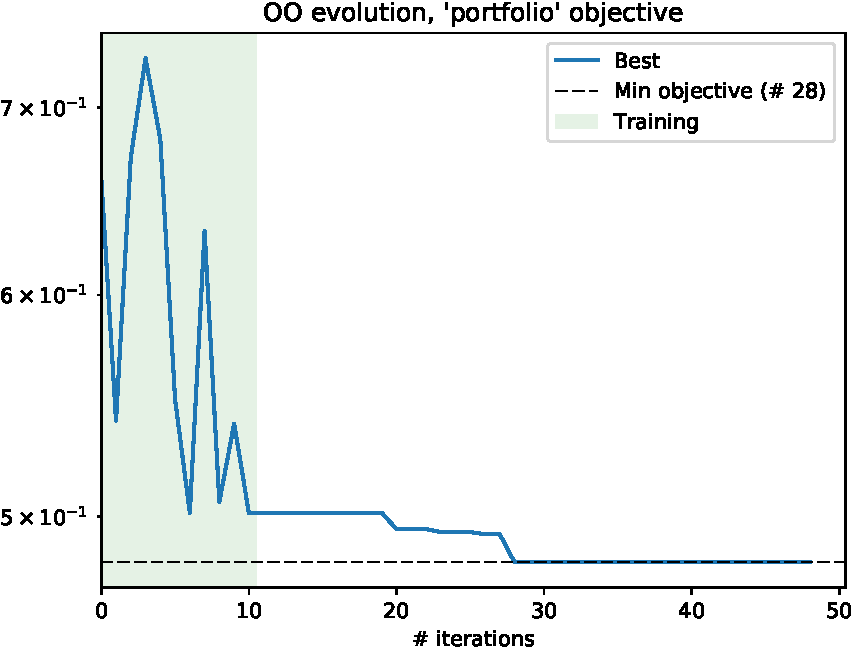
\includegraphics[width=.98\textwidth]{oo/chain-1-report.pdf}
        \end{center}
    \end{minipage}%

%\begin{frame}{}
    %\begin{center}
        %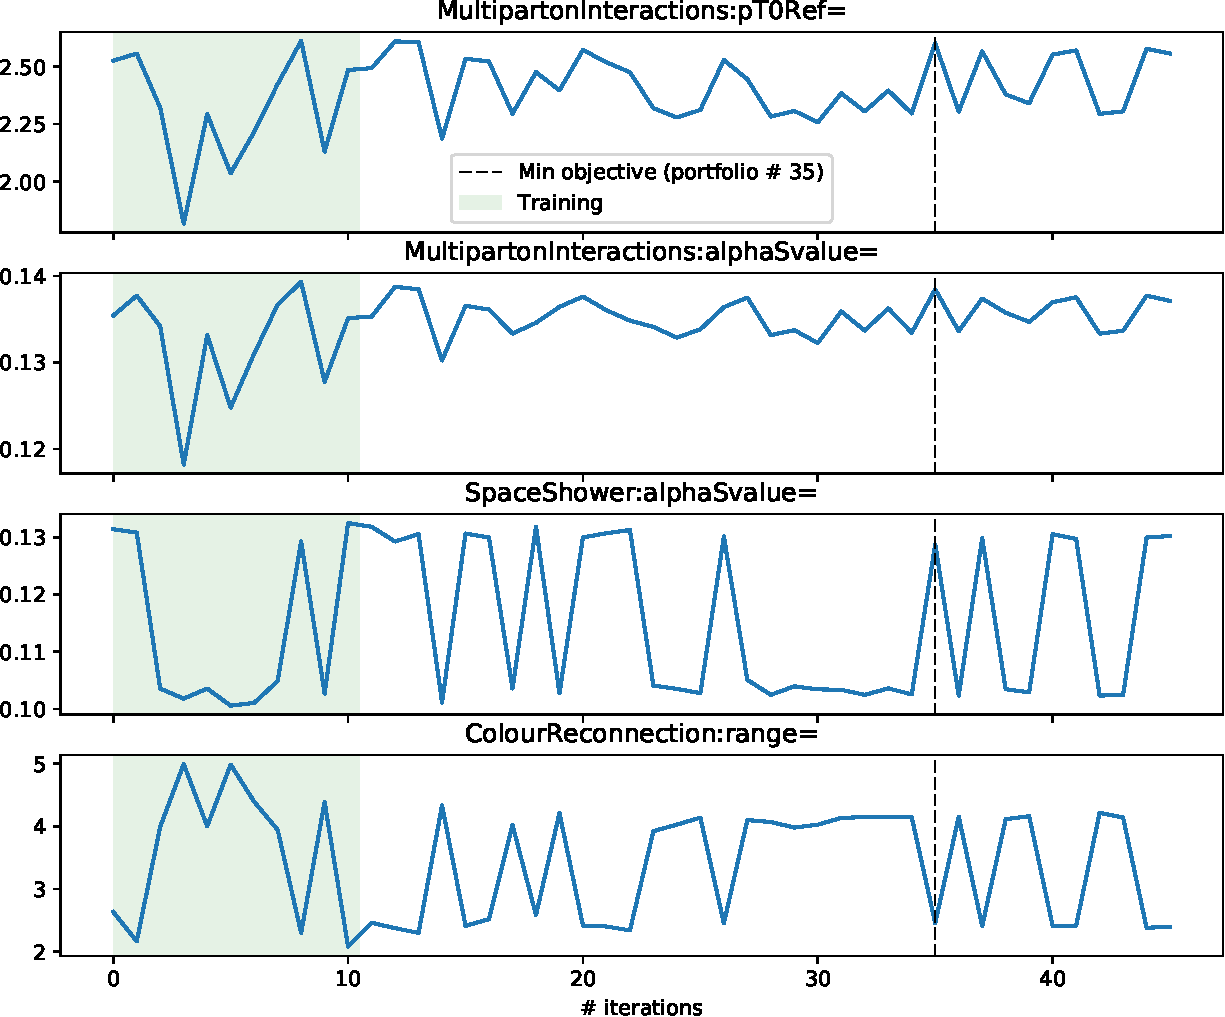
\includegraphics[width=.98\textwidth]{oo/chain-3-report-pevolution.pdf}
    %\end{center}
%\end{frame}
\begin{frame}{Evolution of weights}
    \begin{itemize}
        \item This plot shows the $\left\{w_\mathcal{O}\right\}$  of the outer optimisation
        \item Controlplot to check that weight space is reasonably sampled
    \end{itemize}
    \begin{center}
        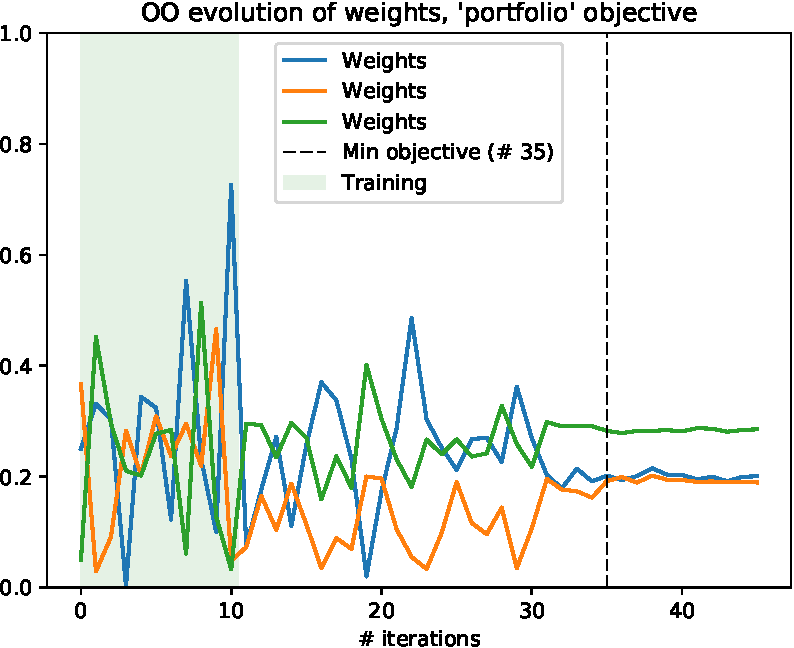
\includegraphics[width=.78\textwidth]{oo/chain-3-report-wevolution.pdf}
    \end{center}
\end{frame}

\begin{frame}{Evolution of inner optimisation}
    \begin{itemize}
        \item This plot shows the \phat of the inner optimisation
        \item Shows the correlation of parameters
    \end{itemize}
    \begin{center}
        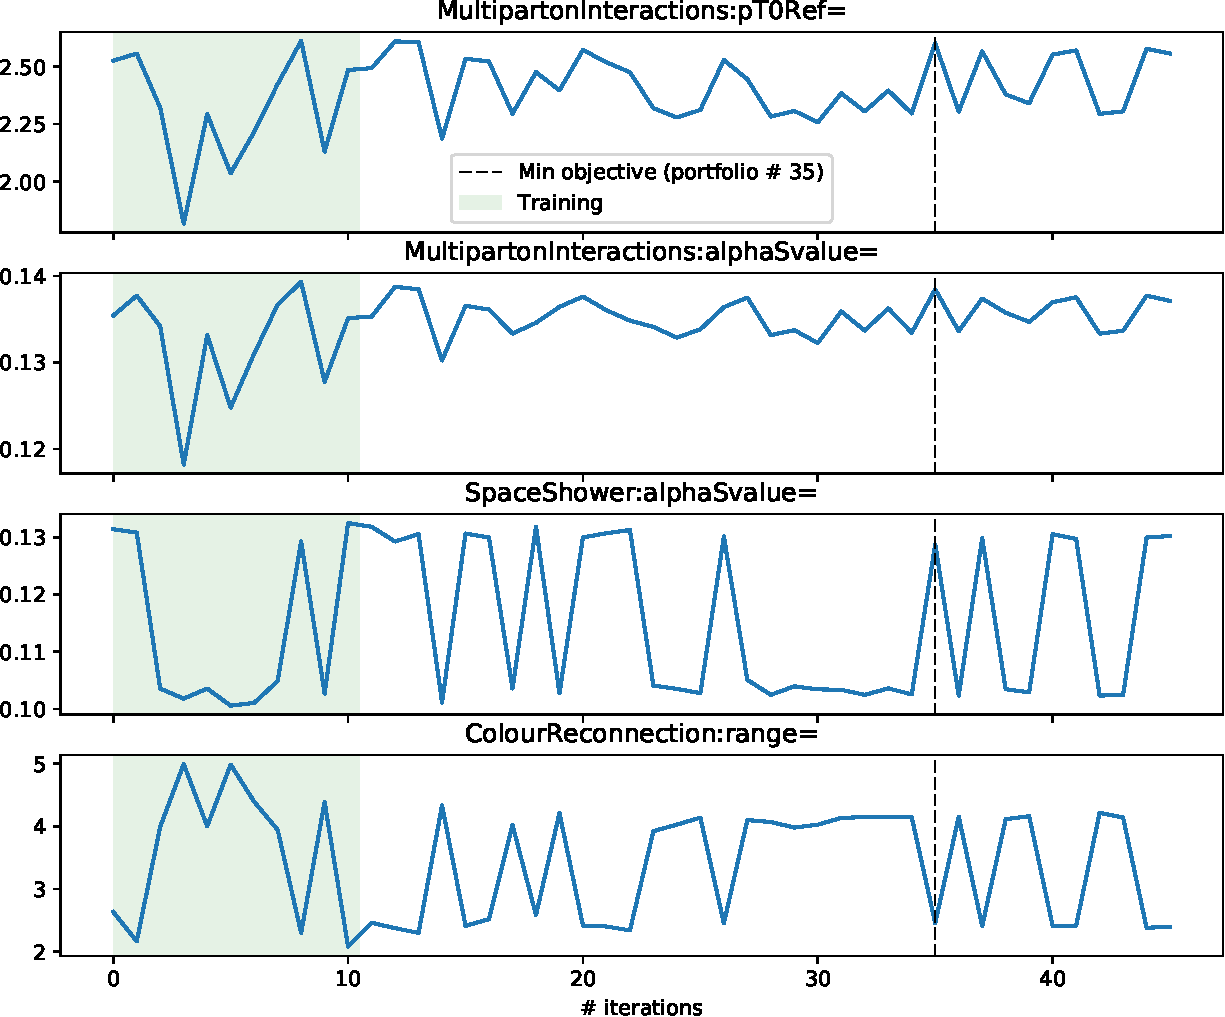
\includegraphics[width=.78\textwidth]{oo/chain-3-report-pevolution.pdf}
    \end{center}
\end{frame}

\begin{frame}{Comparison of results}
    \begin{minipage}{.48\textwidth}%
        \begin{center}
            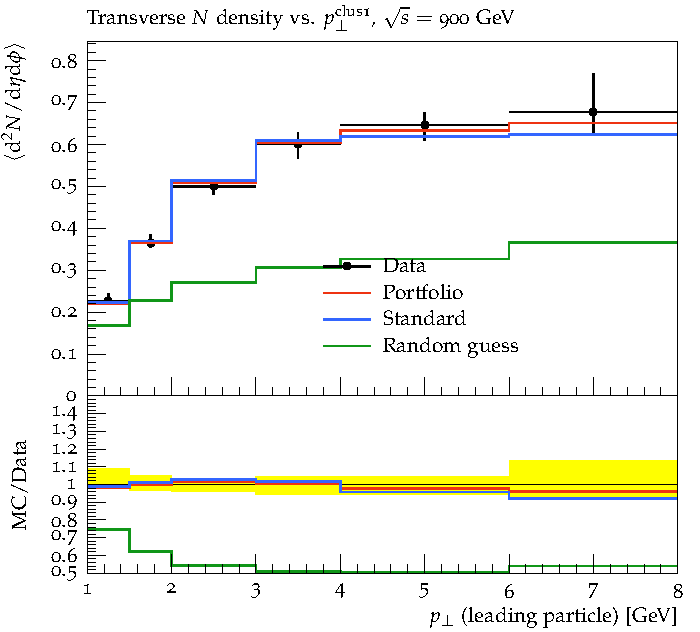
\includegraphics[width=.92\textwidth]{oo/test_cmp_1_std/ATLAS_2011_S8994773/d01-x01-y01.pdf}\\
            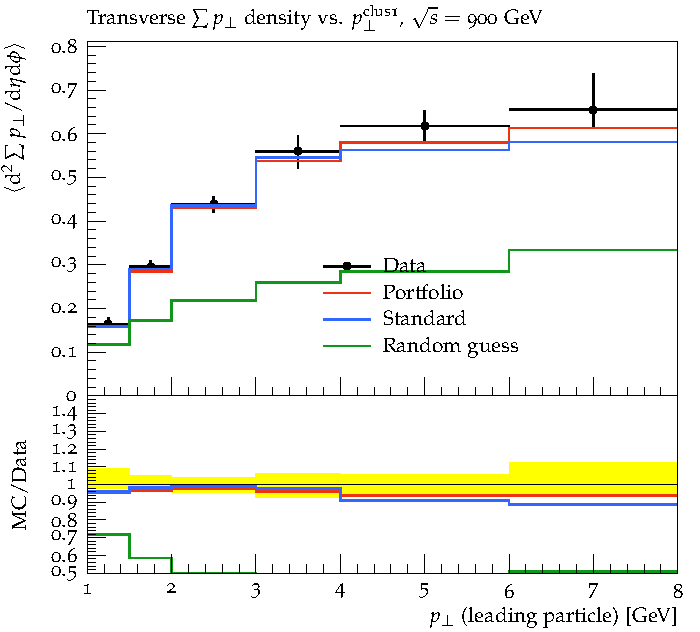
\includegraphics[width=.92\textwidth]{oo/test_cmp_1_std/ATLAS_2011_S8994773/d03-x01-y01.pdf}
        \end{center}
    \end{minipage}%
    \begin{minipage}{.04\textwidth}%
    \end{minipage}%
    \begin{minipage}{.48\textwidth}%
        \begin{center}
            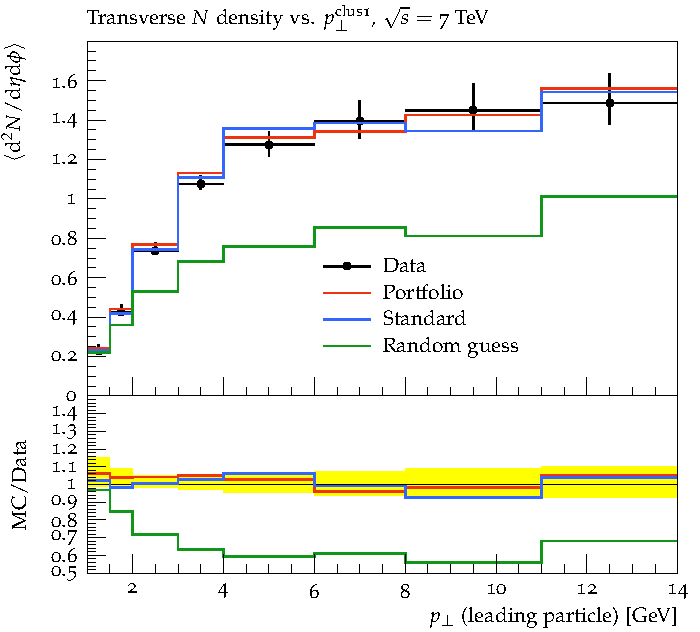
\includegraphics[width=.92\textwidth]{oo/test_cmp_1_std/ATLAS_2011_S8994773/d02-x01-y01.pdf}\\
            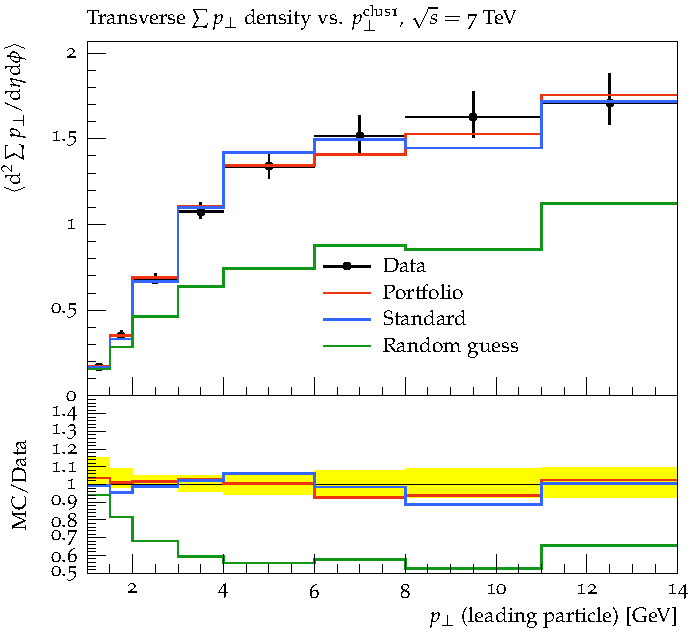
\includegraphics[width=.92\textwidth]{oo/test_cmp_1_std/ATLAS_2011_S8994773/d04-x01-y01.pdf}
        \end{center}
    \end{minipage}%
\end{frame}


\subsection{Multivariate rational approximations}
\label{sec-rapp}

Rational approximations can be seen as natural extensions of the polynomial
approximations used so far in PROFESSOR. Denoting the degrees of the numerator 
and denominator polynomial as $m$ and $n$ respectively, we can formally define
the rational approximation as
\begin{equation}\label{eq:rappdef}
    f^{(m,n)}(p) = \frac{h^{(m)}(p)}{g^{(n)}(p)}.
\end{equation}
Polynomial approximations in this picture are thus simply the class of rational approximations with $n=0$.

\subsection{The algorithm}

For simplicity, we present the algorithm for a one-dimensional parameter space. We are interested in deriving a rational approximation:
\begin{equation}\label{eq:PadeOneD}
  f : \R \to \R, \quad f(p) \simeq \frac{h(p)}{g(p)}
\end{equation}
by fitting the coefficients of $h(p), g(p)$ to data, $(p_l, f(p_l)$. Denoting the polynomials
as
\begin{equation}
  h(p) = a_0 + a_1 p + a_2 p^2 + \ldots + a_m p^m \quad \text{and} \quad
  g(p) = b_0 + b_1 p + b_2 p^2 + \ldots + b_n p^n,
\end{equation}
we observe that we have $K=(m+1)+(n+1)-1$ degrees of freedom (one less, because we can scale
either $a_0=1$ or $b_0=1$ wlog). Assuming that we have $K$ data points, $\left(p_l, f(p_l)\right), l=1,\ldots,K$
that are ``nicely'' chosen, the fitting problem can be written as
\begin{equation}\label{eq:FitPadeOneD}
  f(p_l) =  \frac{h(p_l)}{g(p_l)} \quad \Leftrightarrow \quad g(p_l)f(p_l) =  h(p_l) \quad \forall l=1,\ldots,K
\end{equation}
provided that $g(p_l) \not = 0$. We note, that \eqref{eq:FitPadeOneD} is a square linear
system of equations in $K$ unknowns. To solve this system, we provisionally add coefficients
up to order $K$ to $h(p)$ and $g(p)$ (which we will enforce to be zero later). Thus, we write
the polynomials as
\begin{equation}
  \begin{array}{rcl}
    h(p) & = & a_0 + a_1 p + a_2 p^2 + \ldots + a_m p^m + \ldots + a_K p^K \\
    \text{and} & & \\
    g(p) & = & b_0 + b_1 p + b_2 p^2 + \ldots + b_n p^n + \ldots + b_K p^K.
  \end{array}
\end{equation}
We let the Vandermonde matrix of order $K$ be
\begin{equation}
  V := \left[ \begin{array}{ccccc}
      1 & p_1 & p_1^2 & \ldots & p_1^K \\
        &     &      &        &       \\
      \vdots & \vdots & \vdots &   & \vdots \\
        &     &      &        &       \\
      1 & p_K & p_K^2 & \ldots & p_K^K 
       \end{array}\right]
\end{equation}
and we define the diagonal matrix $F := \text{diag}(f(p_1), \ldots, f(x_K))$, and
vectors of coefficients $a=(a_0,\ldots,a_K)^T$ and $b=(b_0,\ldots,b_K)^T$. Then,
we can write \eqref{eq:FitPadeOneD} compactly as
\[ F V b = V a . \]
If we assume that $V$ is invertible (which imposes a condition on the interpolation points),
then we can rewrite this system as
\[ a = V^{-1} F V b =: Z b , \]
where $Z = V^{-1} F V$. Now recall, that $b_{n+1} = \ldots = b_K = 0$, and denote the first
$n$ components of $b$ by $\hat{b}$, and similarly define $\hat{Z} := Z[:,1:n]$ using Matlab/Python
notation. Then it follows that
\[ a = \hat{Z} \hat{b} ,\]
which is a ``skinny'' system of equations. If we also enforce the condition that
$a_{m+1} = \ldots = a_K = 0$, then we can write this system as
\[ \left(\begin{array}{c}
     a_0 \\ \vdots \\ a_m \\ \hline a_{m+1} \\ \vdots \\ a_K
   \end{array}\right)
   =
   \left[\begin{array}{c} \\ \bar{Z} \\ \\ \hline \\ \tilde{Z} \\ \phantom{+} \end{array}\right]
   \left(\begin{array}{c}
     b_0 \\ \vdots \\ b_n
   \end{array}\right)
   \quad \text{or}\quad \hat{a} = \bar{Z} \hat{b}, \quad \text{and} \quad 0 = \tilde{Z} \hat{b}
\]
We now observe that the last set of equations, $0 = \tilde{Z} \hat{b}$, has $K-m-1=m+n+1-m-1=n$ equations
and $n+1$ unknowns. Thus, if the equations are consistent, we can choose $\hat{b}$ to be a vector that
lies in the null-space of $\tilde{Z}$. Forming an SVD of $\tilde{Z}$
\[ \tilde{Z} = \tilde{U} \tilde{\Sigma} \tilde{V}^T ,\]
we choose $\hat{b} := \tilde{V}[:,n+1]$ as the last singular vector, then obtain $\hat{a} = \bar{Z} \hat{b}$.

The generalisation to multi-dimensional parameter spaces is straight forward.


\subsection{Example}

We consider the function $$f(x) = \frac{1 + x}{1 + x + x^2},\quad
x\in(0,100).$$ The calculation of a rational approximation of type $(m=1, n=2)$
requires the determination of $N_\text{coeff}=6$ coefficients, which is the
same number of coefficients required to build a $5^\text{th}$ order polynomial
in 1 dimension.  Both approximations to the same input data are shown in
\figref{fig:cmp}. The qualitative gain when using rational approximations is
quite evident. Rather importantly for physics use-cases, where purely positive
definite quantities are encountered frequently, we observe that the polynomial
approximations have a tendency to oscillate, leading to negative predictions
which can be unphysical therefore making the application of the latter at least
questionable.

\begin{figure}
    \begin{minipage}{.48\textwidth}%
        \begin{center}
            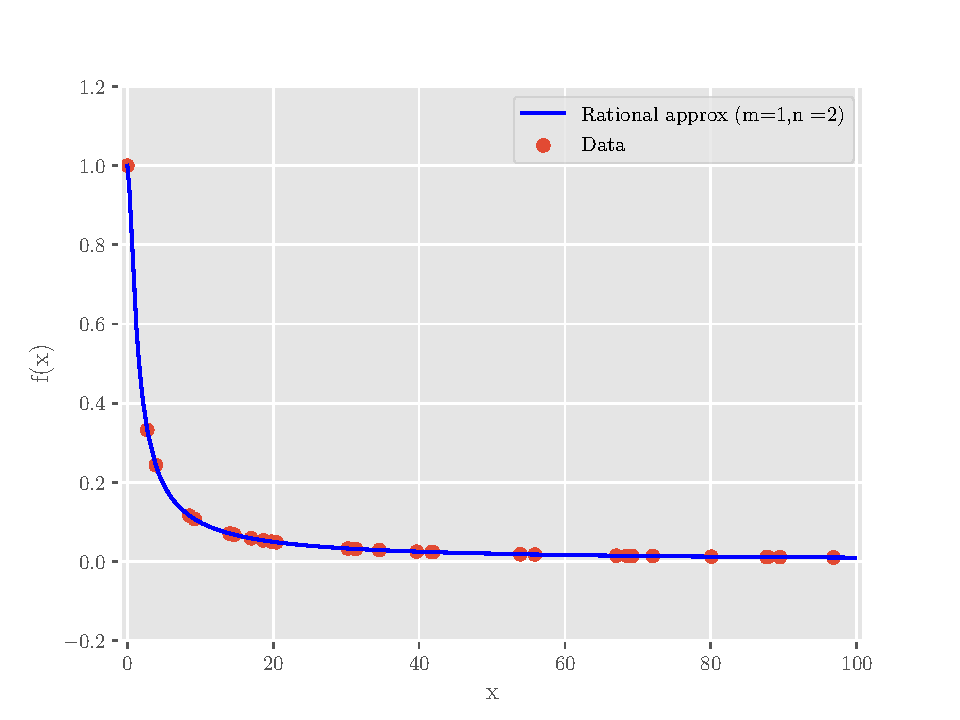
\includegraphics[width=.98\textwidth]{code/test04_01_2.pdf}
        \end{center}
    \end{minipage}%
    \begin{minipage}{.04\textwidth}%
    \end{minipage}%
    \begin{minipage}{.48\textwidth}%
        \begin{center}
            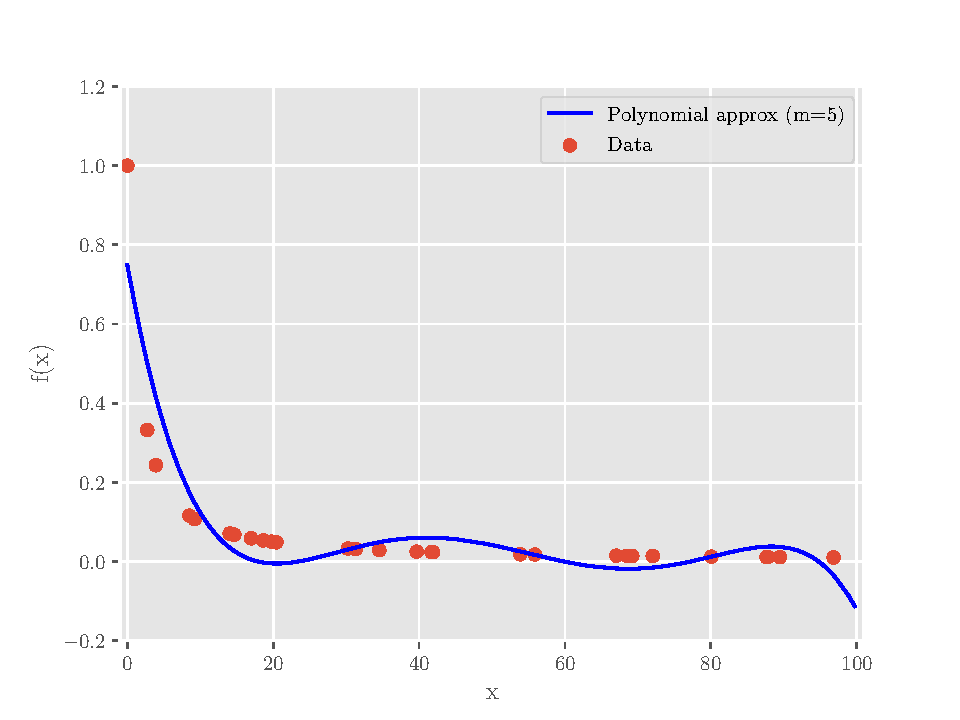
\includegraphics[width=.98\textwidth]{code/test04_05_0.pdf}
        \end{center}
    \end{minipage}%
    \centering
    \caption{Comparison of rational and polynomial approximation to input data
    that exhibits traits of a rational function. Left: rational approximation
with 6 coefficients. Right: polynomial approximation with 6 coefficients.}
    \label{fig:cmp}
\end{figure}






%
\section{Section title}
\label{sec-1}
For bibliography use \cite{RefJ}
\subsection{Subsection title}
\label{sec-2}
Don't forget to give each section, subsection, subsubsection, and
paragraph a unique label (see Sect.~\ref{sec-1}).

For one-column wide figures use syntax of figure~\ref{fig-1}
\begin{figure}[h]
% Use the relevant command for your figure-insertion program
% to insert the figure file.
\centering
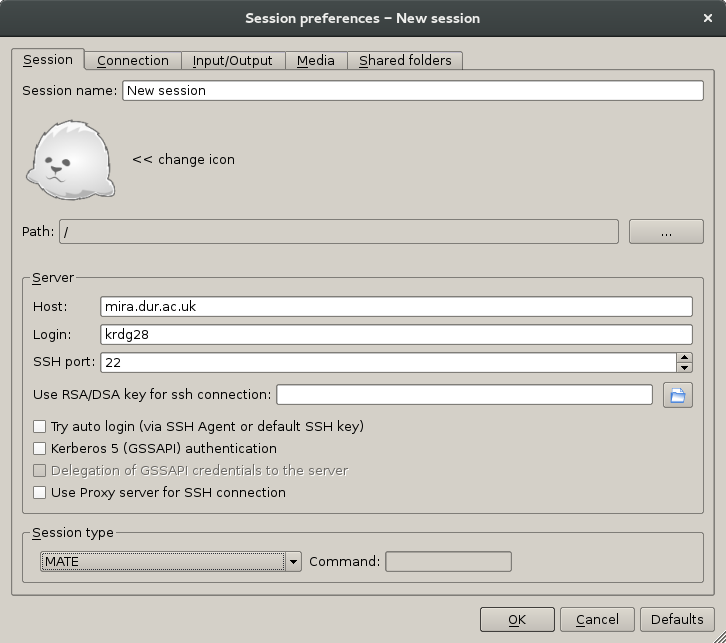
\includegraphics[width=1cm,clip]{tiger}
\caption{Please write your figure caption here}
\label{fig-1}       % Give a unique label
\end{figure}

For two-column wide figures use syntax of figure~\ref{fig-2}
\begin{figure*}
\centering
% Use the relevant command for your figure-insertion program
% to insert the figure file. See example above.
% If not, use
\vspace*{5cm}       % Give the correct figure height in cm
\caption{Please write your figure caption here}
\label{fig-2}       % Give a unique label
\end{figure*}

For figure with sidecaption legend use syntax of figure
\begin{figure}
% Use the relevant command for your figure-insertion program
% to insert the figure file.
\centering
\sidecaption
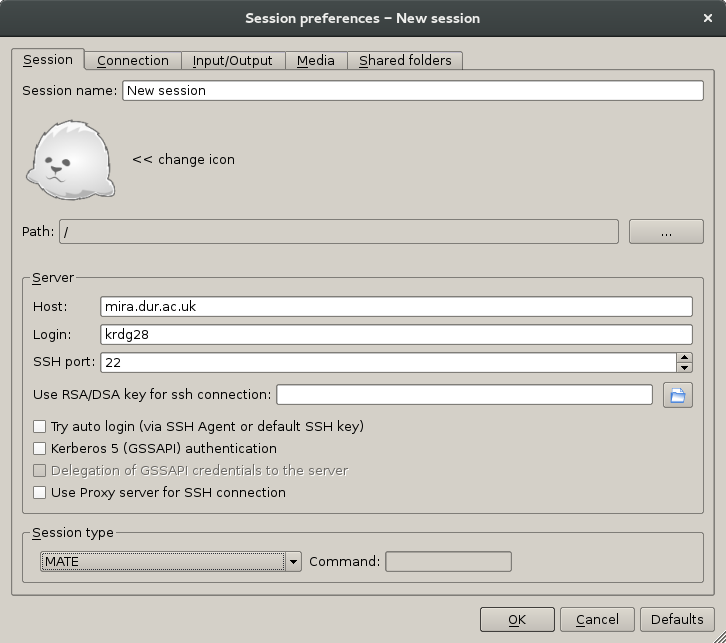
\includegraphics[width=5cm,clip]{tiger}
\caption{Please write your figure caption here}
\label{fig-3}       % Give a unique label
\end{figure}

For tables use syntax in table~\ref{tab-1}.
\begin{table}
\centering
\caption{Please write your table caption here}
\label{tab-1}       % Give a unique label
% For LaTeX tables you can use
\begin{tabular}{lll}
\hline
first & second & third  \\\hline
number & number & number \\
number & number & number \\\hline
\end{tabular}
% Or use
\vspace*{5cm}  % with the correct table height
\end{table}


\section{Summary and outlook}
We presented recent progress in the methodology of of Monte-Carlo event-generator tuning.

%
% BibTeX or Biber users please use (the style is already called in the class, ensure that the "woc.bst" style is in your local directory)
 \bibliography{references.bib}

\end{document}

% end of file template.tex
